\documentclass[mim_thesis.tex]{subfiles} 
\begin{document}

In this chapter will be presented the materials and respective methods used to develop the script, including the system architecture, user stories and use cases. Also, an analysis of the provided repository was done, for comparison of compliant archetypes between the local repository and the international CKM.\\

The provided local repository with artifacts was hosted at GitLab. Is a private repository that needs authentication to access the information inside of it. The REST API provided by this service was in version v4. The comparison repository (openEHR CKM) is publicly accessible and is hosted on GitHub. A REST API is also provided by this service and authentication is not necessary to access to repositories content. This repository is a mirror of all the content posted at \url{http://www.openehr.org/ckm/}. To test the REST API calls in both repositories was used Postman, which is a tool for prototyping and testing HTTP API's with a lot of testing features and with user friendly GUI. To get archetypes from repositories and expose them in a create and edit environment, was used ADLDesigner and some REST API calls from it, that will be explained in more detail bellow. The script will run along with this web tool, since it is dependent from its REST API calls to GitLab repository and require the same credentials to log in and retrieve the hosted archetypes and templates list. For script development was used the Visual Studio Editor from Microsoft and the code for the script was written in Angular 2/Typescript, a variant from Javascript. To host it as a live demo, was used StackBlitz, an online IDE for web applications that is powered by Visual Studio Code (Microsoft) and it is free to use. Moreover, for algorithms flowchart, UML and use cases, was used Camunda Modeler, StarUML and Visual Paradigm. \\

List of links of software used and repositories: 
\begin{itemize}[noitemsep]
\item \textbf{Internal/local repository:} \url{https://gitlab.marand.si/ThinkRegistry/achf/ckm}
\item \textbf{openEHR international CKM GitHub mirror repository:} \url{https://github.com/openEHR/CKM-mirror}
\item \textbf{Postman:} \url{https://www.getpostman.com/}
\item \textbf{ADL Designer:} \url{https://ehrscape.marand.si/designerv2/#/designer/login} (web tool), \url{https://github.com/openEHR/adl-designer} (source code)
\item \textbf{Visual Studio Code:} \url{https://code.visualstudio.com/}
\item \textbf{Angular 2:} \url{https://angular.io/}
\item \textbf{TypeScript:} \url{http://www.typescriptlang.org/}
\item \textbf{StarUML:} \url{http://staruml.io/}
\item \textbf{Camunda Modeler:} \url{https://camunda.com/products/modeler/}
\item \textbf{Visual Paradigm online:} \url{https://online.visual-paradigm.com/}
\item \textbf{StackBlitz:} \url{https://stackblitz.com/}

\end{itemize}


\section{Analysis of archetype content from local repository and comparison with openEHR CKM repository}
Before starting developing the script, an analysis of the provided repository was made. This analysis consisted on a direct comparison between the version, versioning parameters and content of archetypes inside of this local repository in GitLab with the archetypes from the international openEHR CKM hosted on GitHub. The local repository had 41 archetypes and the primary search was made by archetype name on both repositories. For each one of these archetypes was given a status to define the conformity with openEHR CKM: 

\begin{itemize}[noitemsep]
\item \textbf{"Outdated"} in case of versioning parameters (Major Version, revision, archetype UID, MD5-CAM) and content inside of the archetype being different in both repositories;
\item \textbf{"Not found"}, if the archetype in the local repository was totally changed by another one on the international openEHR CKM, but with similar content, or even if this archetype does not exist anymore on the international CKM - case of archetype specializations that lost connection with the parent archetype;
\item \textbf{"Internal"}, which is the case of creation of new archetypes that needs to meet certain clinical needs and are not present on the international CKM or when they are specialized to meet some local or national requirement;
\item \textbf{"Compliant"}, when the archetype has the same versioning parameters (Major Version, revision, archetype UID, MD5-CAM) and content are similar in both repositories, which means that has the latest version from the international CKM;
\end{itemize}

It was expected to have some outdated archetypes during the analysis, since it is a normal behavior in developing area - with time changes are made and \textit{bugs} can be found. In the next table is possible to see the results of this comparison between both repositories. The full analysis can be checked in the annexe 1 from chapter 12 of this dissertation.

\begin{table}[H]
	\centering
	\caption{Summary of archetype comparison analysis from the provided CKM repository with GitHub mirror of openEHR international CKM (June 2018) (n=41)}
	\label{tab:repos_comp}
	\begin{tabular}{lll}
		\toprule[2pt]
		\multicolumn{3}{r}{\textbf{ Total (n=41) }} \\
		\cmidrule(r){2-3}
		\textbf{Archetype Status}   & \textbf{n} & \textbf{(\%)} \\
		\midrule[2pt]
		\textbf{Outdated } & 12 & (29,27) \\
		\midrule
		\textbf{Internal } & 16 & (39,02) \\
		\midrule
		\textbf{Not found } & 3 & (7,32) \\
        \midrule
		\textbf{Compliant } & 10 & (24,39) \\
		\bottomrule[2pt]
	\end{tabular}
\end{table}

Although it is a repository with a high percentage of internal archetypes due to local or national requirements, which are not present in the international CKM, a lot of archetypes are outdated too. Some of them were downloaded to the local repository in November 2016 and since that date, there was no verification of new versions of archetypes from the international CKM. This can result in errors that can still exist in the local repository, that most probably were fixed on the international 
CKM, or even additional content that would enrich the local archetypes. Also, having a repository with these characteristics is not the aim of openEHR ideals, where less than \( \frac{1}{4} \) of the artifacts are compliant with the international CKM. To manually verify same archetypes on both repositories, side by side and check all the content and versioning parameters took around nine hours to complete. 

\subsection{Other Findings between analyzed repositories}
During the analysis of both repositories, some not expected issues have been found, that compromise the correct versioning of those resources due to some error or bug during the implementation management.

\begin{itemize}[noitemsep]
\item From local repository:
\begin{itemize}[noitemsep]
\item Archetypes with the same content, but with different MD5 hash. Those can be due to some error from previous versions of ADL Designer, where this resources have been modeled or by some hand-made change on a text editor and then uploaded again to the local CKM. 
\item Some of the updated archetypes presented minor changes that did not include any change on the MD5 hash parameter, which should not happen. If there is a change in the archetype, even by one character, the MD5 hash should change, since it is created from all the content inside of the archetype.
\item Archetypes that have been codified with build\_uuid instead of build\_uid in the local repository, probably due to some implementation on ADL Designer, for example, the case of \textit{openEHR-EHR-OBSERVATION.body\_weigh} archetype.

\end{itemize}
\item From openEHR CKM mirror at GitHub:
\begin{itemize}[noitemsep]
\item Archetypes that exists on openEHR CKM, but are not mirrored to the GitHub repository, e.g.: \textit{openEHR-EHR-CLUSTER.address\_isa} and \textit{openEHR-EHR-CLUSTER.healthcare\_provider\_parent}.
\item Case of archetypes that have been renamed and lost connection to the previous resource, although they still have the same content and versioning parameters, e.g.: \textit{openEHR-EHR-CLUSTER.timing\_nondaily} and the previous \textit{openEHR-EHR-CLUSTER.timing\_repetition}, or the case of the \textit{openEHR-EHR-OBSERVATION.indirect\_oximetry}, with the previous name \textit{openEHR-EHR-OBSERVATION.pulse\_oximetry}. Since that change of the archetype name provokes a change on the achetype uid, it is complicated for a repository manager to follow the changes made, since the tracking from these archetypes is lost when the uid is changed. If the manager is not checking constantly the openEHR CKM news or the openEHR CKM twitter account, it is tricky and even more time consuming to know what changed and when.
\item Archetypes that are specialized from other archetypes (parents) and the those archetypes have been updated to newer versions or deleted from the repository, which make the connection between them lost.
\end{itemize}
\end{itemize}

\section{Software Engineering}
When designing any type of software, it is necessary to know what are the requirements and needs for correct implementation. Making an user story and a use case of what will be developed in this dissertation can help to understand it in a much better way. These two approaches contain a set of narratives of real situations inside of the problem domain and describe the work flow in the perspective of one or more users of the system.  

\subsection{User story and use case}

A simple example of an use case can be described by an application for medication prescription that is being developed. This application can be used by the physician and patient, where the physician has the possibility to choose instructions that can be sent to the patient, with information about how the medication should be taken and how many times per day it should be done. 

For this, an archetype to define "daily timing" with the times per day (or day parts) was downloaded in December 2017 from the international CKM to the local repository where the application is being developed. This archetype was updated on the international openEHR CKM in January 2018 to correct a mistake on the "magnitude" parameter, that defines and counts how many times per day exists. For example, a day can be divided by morning, moon, afternoon and evening and the sum of all of these events is four, which means that the magnitude value should be at least four. On the outdated archetype ADL that was being used inside of the application under development, the magnitude was defined as "<|0.0..1.0|>", that means the occurrence value can only be 0 or 1. 

Because of this, when the information was inserted in the form by the user (physician) and sent to the server, with more than one day part per day, the archetype logic did not accept that value and it automatically threw an error describing that the added value was not supported. The updated archetype, had defined for magnitude "<|>=1.0|>", which means bigger or equal than 1. This means that this outdated archetype needs to be urgently substituted by the new version on the local repository. In the figure \ref{fig:server_arch_error} can be seen the error threw by the EHR server for the archetype magnitude item, when the parts per day were bigger than one.

\begin{figure}[H]
	\centering
    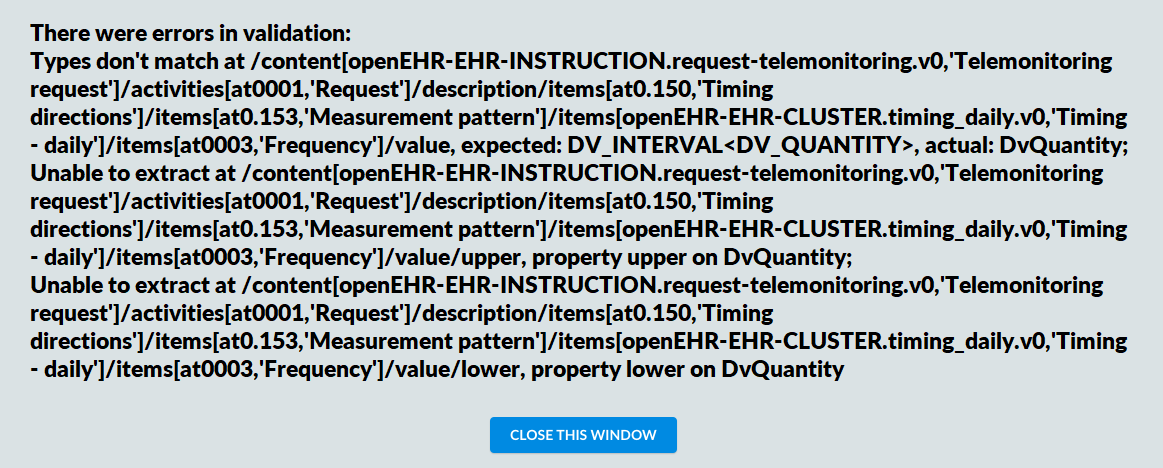
\includegraphics[width=1\textwidth]{img/server_error.PNG}
	\caption{Server error on a under development application by wrong archetype logic (Outdated archetype on local repository)}
	\label{fig:server_arch_error}
\end{figure}

If a experienced openEHR clinical modeler is used to these type of errors, it can be corrected quickly. Usually, if detected in a earlier stage by constant checking for updates on openEHR CKM, can save several time and money on projects.

After some analysis of the CKM repositories users, was defined that the usual user of the script to update the archetypes would be the person responsible for taking care of the governance of the local openEHR artifacts repository on their respective project, role usually performed by a clinical modeler, health informatician or even a programmer (when access to the first two are not available). It starts with one of these users being the "CKM repository owner", creating an account on ADL Designer web application and login on that application. After that, is necessary to create the desired repository connector and connect it to the local repository, which can be from a local computer folder or from an online repository. After the account and repository were created, a login with the same credentials and repository id from ADL Designer needs to be inserted on the login section of the script page ,and if the user is authenticated successful, the script will run the code and a table with a list of archetypes and templates from that repository will be presented. If there are updates, those will appear together in a column with the alert of an outdated or compliant archetype with the openEHR CKM mirror on GitHub, for each element from those lists. A link that retrieve the actual archetype RAW form (ADL) from the openEHR CKM mirror on GitHub should be click-able. Then, if the user wants to download this new archetype to his computer, he can use a tool for comparison like Tortoise SVN, that will show the difference between the new archetype and the old archetype hosted in the local repository. This part needs to be done manually by the user. 

\begin{figure}[H]
	\centering
    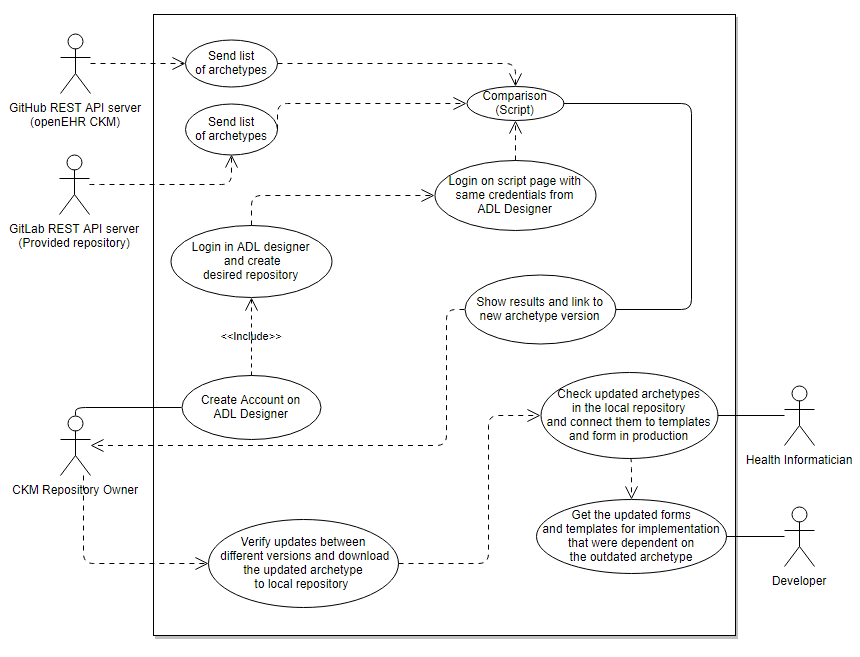
\includegraphics[width=0.95\textwidth]{img/usecase2.PNG}
	\caption{Use case scenario}
	\label{fig:use_case}
\end{figure}


\newpage
\section{ADL Designer}
ADL Designer is a open source web based tool developed by Marand d.o.o. for implementation of modeling tools used in development of openEHR artifacts. Is mostly written on JAVA and JavaScript, with a web interface based on jQuery and Bootstrap 3 frameworks. It has full compatibility with the OET files from the previous openEHR tools by Ocean Informatics and also to version 1.4 of archetypes and templates. Is composed by two main modules, the Archetype Editor and Template Editor. \\

For using this tool, is mandatory to have an account to login. Currently it provides a free access for testing with a default "test" account. After login is necessary to add a web repository or a local folder repository. One of the most interesting features from ADL Designer is that it can be connect to inumerous repositories hosted in different GIT providers, either online or local, such as GitHub, GitLab, Bitbucket, Dropbox, Google Drive, OneDrive or at a local GIT folder in a single computer, allowing the possibility to work on top of each one of them. With this, is possible to edit archetypes and templates from these repositories and directly save the changes made on the repositories again, having the history of all these changes in one place and the possibility to rewind in case of sudden lost of files.

\begin{figure}[H]
	\centering
    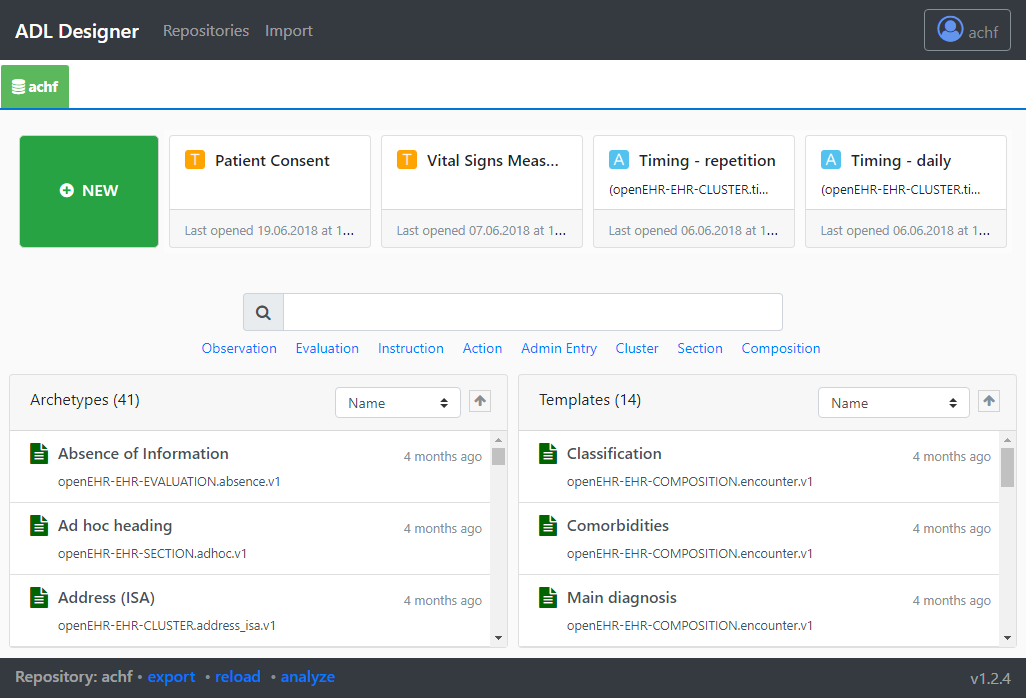
\includegraphics[width=1\textwidth]{img/adldesigner.PNG}
	\caption{ADL Designer (Marand d.o.o.)}
	\label{fig:adldesigner}
\end{figure}

Also, it gives the option of exporting the content from the added repository and analyze the content, like retrieving the amount of normal and specialized archetypes, getting the information if some parent archetype that was used for specialization is missing from the repository, getting the list of clinical terminologies bindings used on each archetype and by parsing them it shows if there are misleading in some terms or constrains, or if \textit{RMtype} slots are not filled on the respective templates. It is in constant development and will support new features in a near future.  \\

The source code can be found at \url{https://github.com/openEHR/adl-designer}. 

\subsection{Archetype Editor}
With this module is possible to edit, specialize, save, import and export archetypes in the ADL2 version. It offers an improved and user friendly GUI comparing with all the other openEHR modeling tools and more exporting formats, such as OPT, OET, xmind (mindmap) and Fileset.

\begin{figure}[H]
	\centering
    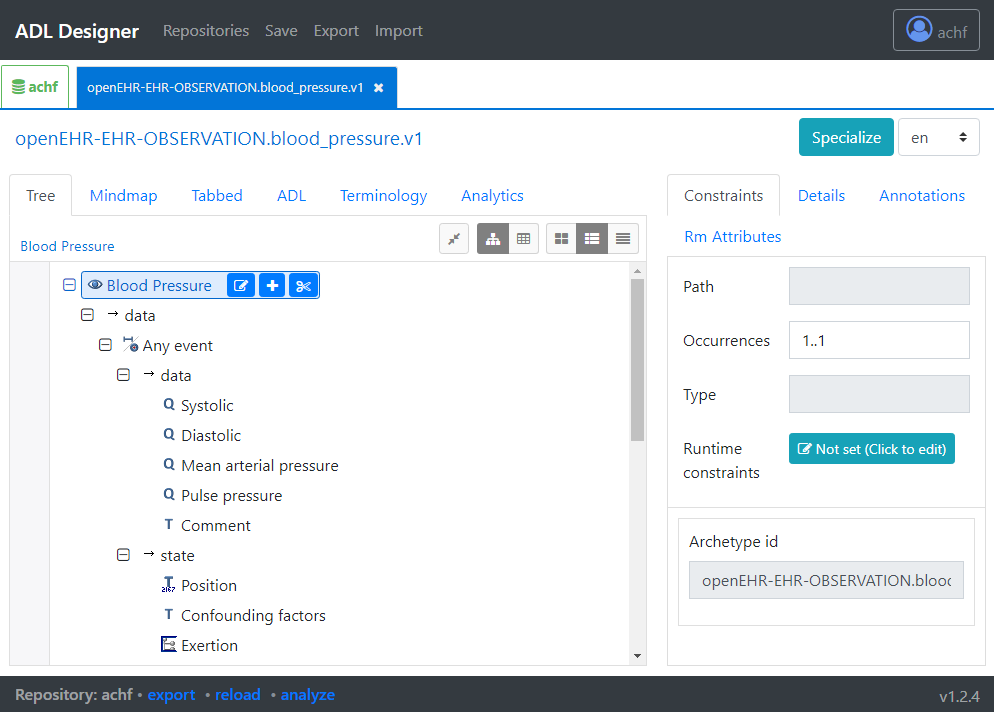
\includegraphics[width=1\textwidth]{img/archetype_editor_adldesigner.PNG}
	\caption{ADL Designer Archetype Editor - Web Interface (Marand d.o.o.)}
	\label{fig:archetypeEditor}
\end{figure}

Architecturally is composed by two different sub-modules, exposed on figure \ref{fig:archetypeEditorArchitecture}, one handled by the browser that allows to see the interface of archetype editor with the help of the "Archetype Object Model" (AOM) and the Reference Model (RM) packages. The AOM is a set of code packages which can be used with archetype parsers and software to manipulate archetypes and it is independent from the web interface. \\
\newpage
It has supported functionality from AOM package for various properties, such as \citep{openEHRALD2016}:
\begin{itemize}[noitemsep]
\item \textbf{AOM.ArchetypeModel} - Wraps AOM of a single archetype, allowing for easier manipulation. It can also manipulate terminology, annotations, constraints, translations, bindings and specialized archetypes;
\item \textbf{AOM.NodeId} - models a single node\_id, such as id1.1.3;
\item \textbf{AOM.RmPath} - models a single rm\_path, such as /data[id3]/items[id4]/value;
\item \textbf{AOM.AmQuery} - enables searching for constraints that match a particular rm\_path;
\item \textbf{AOM.createNewArchetype} - Create a new archetype from scratch, with a provided basic structure based on the Reference Model class;
\item \textbf{AOM.ReferenceModel} - Provides reflection-like functionality for a reference model.
\end{itemize}

The RM takes care of the handling of constrains data types packages, like classes for DV\_DATE, DV\_TEXT, DV\_INTERVAL, DV\_QUANTITY, DV\_TIME and many more. \\ 

The other sub-model is handled by the web server, where the REST calls are being made to the repositories that have been previously connected to ADL Designer over the "Archetype Repository" module. This module makes use of the "adl2-core", a reference implementation of openEHR reference model, archetype model, ADL and AOM2 semantics. Is based on a JAVA library and is the \textit{core} of ADL2 implementations of openEHR. For example, this will allow to parse all the archetypes. \\

\begin{figure}[H]
	\centering
    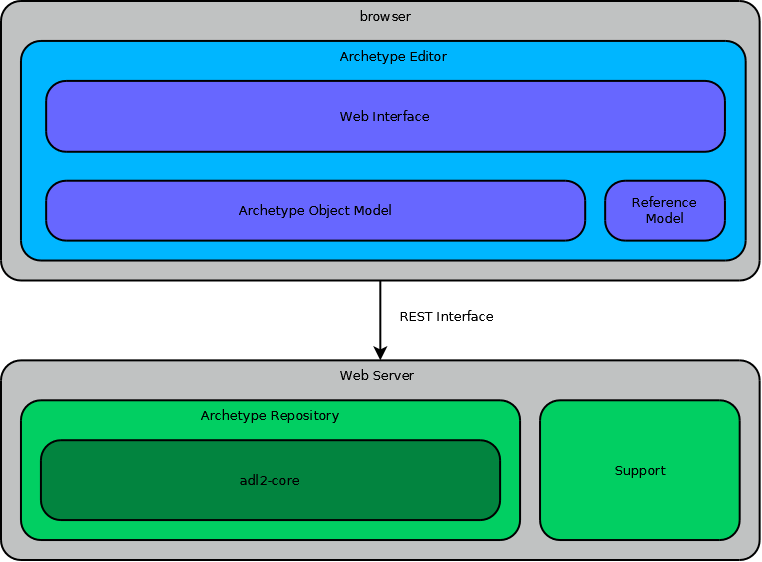
\includegraphics[width=0.80\textwidth]{img/archetype-editor-architecture.png}
	\caption{ADL Designer Archetype Editor - Architecture (Marand d.o.o.)}
	\label{fig:archetypeEditorArchitecture}
\end{figure}

The source code can be found at \url{https://github.com/openEHR/adl2-core/}. 

\newpage
\subsection{Template Editor}

The template editor works in a similar way of Archetype Editor. It uses the same basis and functionality with the two sub-models, browser and web-server, but with major changes on the browser side. It has one more functionality added to the AOM variable: 
\begin{itemize}[noitemsep]
\item \textbf{AOM.TemplateModel}, which models a template where is possible to add or remove archetypes.
\end{itemize}

All the other functionalities from AOM variable (ArchetypeModel, NodeId, RmPath, AmQuery, ReferenceModel) are inherited from the Archetype Editor model, mentioned previously.

\begin{figure}[H]
	\centering
    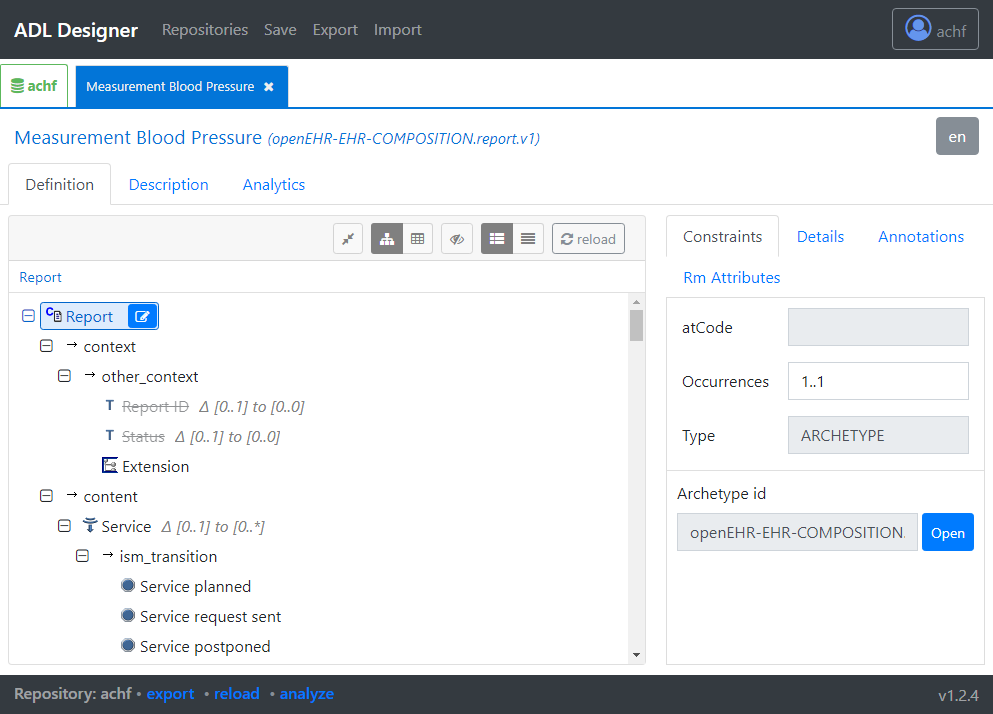
\includegraphics[width=1\textwidth]{img/template_editor_adldesigner.PNG}
	\caption{ADL Designer Template Editor - Web Interface (Marand d.o.o.)}
	\label{fig:templateEditor}
\end{figure}

Some of the features that are possible to be done on this editor are: Adding annotations, making changes to the occurrences of some openEHR template paths, adding external terminology (for example from a URI) or adding local terminology, work on the desired language present on the composition archetype and in the archetypes added as a content in the main template.

Along with the "Archetype Repository" module, it also has the "Template Repository" modules in the web server side, that make accesses by REST API calls to the repository where the content is allocated and retrieves the list of templates. Besides that, it allows to load, edit and save the templates back to that repository. In the figure \ref{fig:templateEditorArchitecture} is possible to see the architecture model. 

\begin{figure}[H]
	\centering
    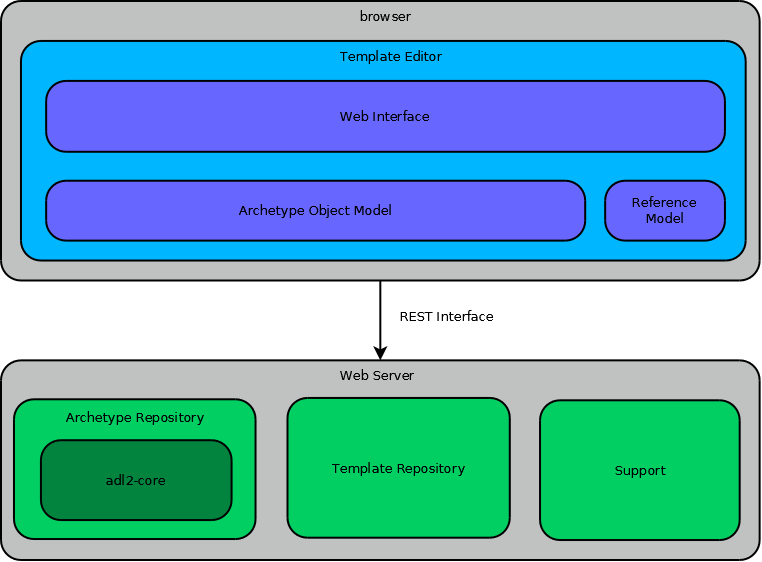
\includegraphics[width=0.85\textwidth]{img/template-editor-architecture.png}
	\caption{ADL Designer Template Editor - Architecture  (Marand d.o.o.)}
	\label{fig:templateEditorArchitecture}
\end{figure}

\section{Angular 2}
Angular 2 is a open-source web application platform made by Google that relies on front-end for building client-side applications in \ac{HTML} and it is based on TypeScript \citep{angular}.

Is fully re-written from its predecessor, the Angular JS (JavaScript). The developed script from this dissertation was written with using framework, since it can provide almost all the needed functionalities out of the box, like the HTTP client that allows to interact with the REST API calls from both openEHR resources repositories and dependency injection without having to worry with external libraries, since this framework bring a bigger part of them.

It is composed by modules, components, services and dependency injection. 
Angular allows to construct modular applications and it has also a modular system - the NgModule, which contains code for the application domain and explain how the application parts fits together. It contains a decorator called @NgModule that has the metadata and properties to describe the module like: imports, providers, declarations, exports and \textit{bootstrap}. These properties can be seen in table \ref{tab:ngmoduleexample}. 

The components are what controls the view of what will appear on the screen. These components can be created, updated or destroyed depending on the user movement through the application depending on the lifecycle function chosen.   

\begin{table}[H]
\caption{Example of \textit{NgModule} and \textit{Component} decorators at app.module.ts and app.component.ts files from the developed script.}
\label{tab:ngmoduleexample}
\centering
\begin{tabular}{l}
\toprule[2pt]
\begin{lstlisting}[language=XML]
##################### app.module.ts #####################

import { BrowserModule } from '@angular/platform-browser';
import { NgModule } from '@angular/core';
import { HttpClientModule } from '@angular/common/http';
import { getArchetypesFromADL } from './app.service'
import { AppComponent } from './app.component';

@NgModule(
	{
          declarations: [ AppComponent ],
          imports: [ BrowserModule, HttpClientModule ],
          providers: [ getArchetypesFromADL ],
          bootstrap: [ AppComponent ]
	}
)

export class AppModule { }



##################### app.component.ts ######################


@Component(
    	{
          selector: 'app-root',
          templateUrl: './app.component.html',
          styleUrls: ['./app.component.css'],
          providers: [getArchetypesFromADL]
    	}
)

\end{lstlisting}
\tabularnewline \bottomrule[2pt]
\end{tabular}
\end{table}



\subsection{NPM}
The npm is a \ac{CLI} package manager helper that interacts with a remote registry and downloads automatically or when required the external libraries and plugins for the project that is being developed. Although that are other versions like "\textit{yarn}", the npm was the one chosen for the script due to be easy to use and because it has access to a huge number of packages. For example, it can downloads all the necessary libraries that are necessary from Angular, like "@angular/core" for the Core module or the HTTP client module like "@angular/common/http" for the HTTP requests. 


\subsection{TypeScript}
Typescript is a scripting language that works as a superset of JavaScript and was created by Microsoft. It has more static types, asynchronous functions and tools than JavaScript and it can make type-checking and auto-completion of the code while is being typed. The aim to create this new language was to make the writing code more maintainable in large JavaScript projects.


\section{GitHub OpenEHR CKM Mirror}
OpenEHR foundation hosted at GitHub a mirror from the CKM clinical models at \url{https://www.openehr.org/ckm/}, which automatically updates when changes are made on the CKM trunk. Since it is connected the GitHub, it is possible to use the REST API resources from this service.


\end{document}